%% Standalone figure for the Statistical Mechanics exercises (Quiz 1).
%% Build: pdflatex quiz1_sol_tx.tex  (or run build.sh in this folder)
\documentclass[11pt,tikz,border=2pt]{standalone}
\usepackage{amsmath,amssymb}
\usetikzlibrary{arrows.meta, positioning}
\begin{document}
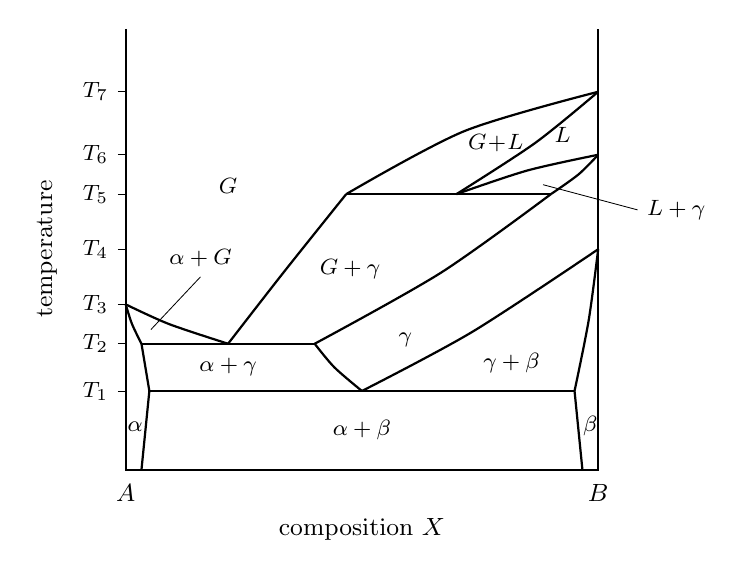
\begin{tikzpicture}[font=\small, >=Latex, line width=0.8pt]
    % frame; T_1 ... T_7 are the crossings of the isobar p_0 in the P-T projection
    \draw (0,5.6) -- (0,0) -- (6,0) -- (6,5.6);
    \foreach \y/\n in {1.0/T_1, 1.6/T_2, 2.1/T_3, 2.8/T_4, 3.5/T_5, 4.0/T_6, 4.8/T_7}
        \draw[dashed, line width=0.3pt] (-0.1,\y) node[left, font=\footnotesize] {$\n$} -- (0,\y);
    % alpha and beta solvus below the eutectoid
    \draw (0.30,1.0) -- (0.20,0);
    \draw (5.70,1.0) -- (5.80,0);
    % three-phase isotherms
    \draw (0.30,1.0) -- (5.70,1.0);      % alpha + gamma + beta (eutectoid)
    \draw (0.20,1.6) -- (2.40,1.6);      % alpha + G + gamma
    \draw (2.80,3.5) -- (5.40,3.5);      % G + L + gamma
    % alpha + gamma region
    \draw (0.30,1.0) -- (0.20,1.6);
    \draw plot[smooth] coordinates {(3.0,1.0) (2.65,1.3) (2.40,1.6)};
    % gamma + beta region, closing at pure B (T_4)
    \draw plot[smooth] coordinates {(3.0,1.0) (4.4,1.75) (6,2.8)};
    \draw plot[smooth] coordinates {(5.70,1.0) (5.88,1.9) (6,2.8)};
    % alpha + G region, closing at pure A (T_3)
    \draw plot[smooth] coordinates {(0.20,1.6) (0.08,1.85) (0,2.1)};
    \draw plot[smooth] coordinates {(1.30,1.6) (0.55,1.85) (0,2.1)};
    % G + gamma region
    \draw plot[smooth] coordinates {(1.30,1.6) (2.0,2.5) (2.80,3.5)};
    \draw plot[smooth] coordinates {(2.40,1.6) (4.0,2.5) (5.40,3.5)};
    % G + L region, closing at pure B (T_7)
    \draw plot[smooth] coordinates {(2.80,3.5) (4.3,4.3) (6,4.8)};
    \draw plot[smooth] coordinates {(4.20,3.5) (5.2,4.15) (6,4.8)};
    % L + gamma region, closing at pure B (T_6)
    \draw plot[smooth] coordinates {(4.20,3.5) (5.1,3.8) (6,4.0)};
    \draw plot[smooth] coordinates {(5.40,3.5) (5.75,3.75) (6,4.0)};
    % region labels
    \begin{scope}[font=\footnotesize]
        \node at (3.0,0.5) {$\alpha+\beta$};
        \node at (1.3,1.3) {$\alpha+\gamma$};
        \node at (4.9,1.35) {$\gamma+\beta$};
        \node at (3.55,1.65) {$\gamma$};
        \draw[line width=0.3pt] (0.32,1.78) -- (0.95,2.45) node[above] {$\alpha+G$};
        \node at (2.85,2.55) {$G+\gamma$};
        \node at (1.3,3.6) {$G$};
        \node at (4.7,4.15) {$G\!+\!L$};
        \draw[line width=0.3pt] (5.3,3.62) -- (6.5,3.3) node[right] {$L+\gamma$};
        \node at (5.55,4.25) {$L$};
        \node at (0.12,0.55) {$\alpha$};
        \node at (5.9,0.55) {$\beta$};
    \end{scope}
    \node[below] at (0,-0.05) {$A$};
    \node[below] at (6,-0.05) {$B$};
    \node[below=14pt] at (3,0) {composition $X$};
    \node[rotate=90] at (-1.0,2.8) {temperature};
\end{tikzpicture}
\end{document}
